
\documentclass[10pt]{article} % For LaTeX2e
% \usepackage{tmlr}
% If accepted, instead use the following line for the camera-ready submission:
\usepackage[preprint]{report}
% To de-anonymize and remove mentions to TMLR (for example for posting to preprint servers), instead use the following:
%\usepackage[preprint]{tmlr}

% Optional math commands from https://github.com/goodfeli/dlbook_notation.
% \input{math_commands.tex}
\usepackage{amsmath,amsfonts,bm}

\usepackage[
colorlinks=true,
pagebackref, 
citecolor=blue, 
pdfpagelabels,
pageanchor=true,
plainpages=false,
bookmarks,
bookmarksnumbered,]
{hyperref}
\usepackage{url}
\usepackage{graphicx}
\usepackage[ruled]{algorithm2e}
\usepackage{tikz}
\usepackage{float}


\title{Proximal Algorithms for Basis Pursuit Denoising}

% Authors must not appear in the submitted version. They should be hidden
% as long as the tmlr package is used without the [accepted] or [preprint] options.
% Non-anonymous submissions will be rejected without review.

\author{\name 
    Francis Moran\email
    fdm31@scarletmail.rutgers.edu\\\\
    \name 
    Ali Zafari
    \email
    ali.zafari@rutgers.edu
}

\def\repo{\href{https://github.com/frankiemoran90/convex_term_project}{\textbf{[link]}}}

% The \author macro works with any number of authors. Use \AND 
% to separate the names and addresses of multiple authors.

\newcommand{\fix}{\marginpar{FIX}}
\newcommand{\new}{\marginpar{NEW}}


\newtheorem{theorem}{Theorem}

% \theoremstyle{definition}
\newtheorem{definition}{Definition}[section]

\begin{document}


\maketitle

\begin{abstract}
This paper aims to describe the theory and application of modern proximal optimization algorithms with respect to the Basis Pursuit Denoising problem. First, a look at proximal optimization theory will take place, followed by the construction of fundamental algorithms. Next, the problem statement will be described and potential algorithms will be discussed. Specifically, this paper will focus on three algorithms: Iterative Shrinking Thresholding Algorithm (ISTA), Fast Iterative Shrinking Thresholding Algorithm (FISTA), and Sparse Reconstruction by Separable Approximation (SpaRSA). Experimentation will be performed on a sample image and results will be compared.
\end{abstract}

\section{Introduction}
\subsection{Motivating Proximal Algorithms}
We have seen gradient based algorithms to find solutions of unconstrained minimization problems over the semester \citep{boyd2004convex}. When the objective function is non-smooth (non-differentiable) these algorithms and their convergence analysis are no longer valid. The basic solution when the objective function is still convex but not necessarily differentiable is to use the method of subgradients. Although it fixes the differentiability requirement of gradient-based methods, its notorious slow convergence rate prohibits its practical usage. This disadvantage is where the proximal algorithms shine as they can provide the same convergence rate offered by gradient-based methods for non-smooth convex objective functions \citep{parikh2014proximal}. In the next section we briefly analyze the convergence rate of subgradient methods to motivate the topic of this project.

\subsubsection{Convergence of Analysis of Subgradient Methods}

The subgradient method is the non-smooth version of gradient descent. The basic algorithm is straightforward, consisting of the iterations:
    \begin{align*}
        x_{k+1}=x_k-\alpha_k\Delta x_k
    \end{align*}
    where the $\Delta x_k$ is any member of $\partial f(x_k)$.
\begin{definition}[Subgradient]
    Subgradient of function $f$ at $x$ is a vector $g\in\mathbb{R}^n$ such that
    \begin{align*}
        f(y)\geq f(x)+g^T(x-y) \;\;\forall y\in\mathrm{dom}f
    \end{align*}
    Collection of subradients at $x$ is called the subdifferential at $x$ denoting as $\partial f(x)$.
\end{definition}
The major disadvantage of subgradient methods is their extremely slow rate of convergence. Further, some cases may provide no guarantee for convergence. The next two theorems show this claim, the proofs can be found in \citep{boyd2003subgradient}.

\begin{theorem}[Subgradient Non-convergence!]
    Let $f$ be a convex Lipschitz continuous function with $M>0$. Suppose that step size $\alpha_k=\alpha > 0$ is fixed for all $k$. Then
    \begin{align*}
        f_k^{\text{best}}-f(x^\star)\leq\frac{1}{2\alpha k}\|x_0-x^\star\|_2^2+\frac{\alpha M^2}{2}
    \end{align*}
    \end{theorem}
Subgradient method does not guarantee a decrease in function value at each iteration, so we keep the best after $k^{th}$ iteration, $f_k^{\text{best}}$. For fixed step size, convergence is not guaranteed.

\begin{theorem}[Subgradient Convergence]
    Let $f$ be a convex Lipschitz continuous function with $M>0$. Suppose that step sizes satisfy $\alpha_k\rightarrow 0$ as $k\rightarrow\infty$ and $\sum_{k=1}^\infty\alpha_k=\infty$. Then the achievable rate for a general $f$ is
    \begin{align*}
        f_k^{\text{best}}-f(x^\star)\leq\frac{1}{\sqrt{k}}\|x_0-x^\star\|_2^2+Const.\frac{ M^2\log k}{\sqrt{k}}
    \end{align*}
    \end{theorem}

This convergence rate is slow compared to gradient descent. The choice of step size heavily affects the convergence rate of subgradient method.

\subsection{Search for Acceleration}

To avoid the extremely slow convergence rate of subgradient methods, in cases which the proximal mapping (to be defined in the next section) can be done efficiently proximal algorithms are introduced. These algorithms have similar convergence rates to those of gradient descent methods.\\
It has also been shown that the convergence rate of gradient descent methods can be improved significantly by momentum-based methods. Informally, this involves mixing some history of gradient updates into the current estimate. Using the same gradient descent method but with new updates:
\begin{eqnarray*}
\begin{aligned}
    &y_k = x_k+ \beta_k(x_k-x_{k-1})\\
    &x_{k+1}=y_k-\alpha_k\nabla f(y_k)
    \end{aligned}
\end{eqnarray*}
where $\beta_k=\frac{k-1}{k+2}$.
The next theorem indicates this claim.

\begin{theorem}[Nestrov's Optimal Method]
Let $f$ be a convex $L$-smooth function ($L>0$). Nestrov's updates for suitable choices of step size $\alpha_k$ using gradient-based descent optimization yields \cite{romberg2022}:
    \begin{align*}
        f(x_k)-f(x^\star)\leq\frac{2L}{(k+1)^2}\|x_0-x^\star\|_2^2
    \end{align*}
\end{theorem}

This same idea was explored for proximal algorithms applied to the BPDN problem. The papers \citep{beck2009fast,wright2009sparse} discussed in this project have this goal of accelerating the regular proximal algorithm.

\subsection{Proximal Operators}

Proximal Algorithms are a type of optimization algorithms that excel at solving non-smooth and constrained convex optimization problems. The fundamental mechanism behind these algorithms is shown in the proximal operator $\mathbf{prox}_f$. The proximal operator maps a point $v \in \mathcal{R}^n$ to $x \in \mathcal{R}^n$ based on the function value $f(x)$ and the proximity between $v$ and $x$.  

Let $ {f} : \mathcal{R}^n \xrightarrow{} \mathcal{R} \cup \{ + \infty \}$ be a closed convex function with domain 
\begin{align*}
    \mathbf{dom}{f} = \{ x \in \mathbf{dom}{f}  \ | \  {f}(x) < + \infty \}
\end{align*}

The function $f$ will have the extended value of $+ \infty$ for all $x \notin \mathbf{dom} f$. The proximal operator $\mathbf{prox}_f$ is then given by:

\begin{align*}    
\mathbf{prox}_{\lambda f} (v) = \underset{x}{\arg\min} (f(x) + \frac{1}{2 \lambda} \| x - v \|_2^2)
\end{align*}

\noindent where $\lambda$ is a parameter that determines the weight of the proximity term.

The proximal operators mapping can be described in two cases. In case one, $v \notin \mathbf{dom} f$. Here, the extended value of $f$ will ensure the mapped point $x \in \mathbf{dom}{f}$. In the other case, $v \in \mathbf{dom}{f}$. Now the proximal operator will map $x$ such that $f(x) \leq f(v)$. 

It should also be noted that when $f(x) = f(v)$, or the operator returns a fixed point, then $x$ (or $v$) minimizes $f$. In other words, $x^*$ is a minimizer of $f$ if and only if: 

\begin{center}
    $x^* = \mathbf{prox}_{\lambda f} (x^*)$
\end{center}

\noindent This property of proximal operators is very useful in algorithm development. 

Another property that will be useful is the evaluation of a proximal operator $\mathbf{prox}_{\lambda f}$ when $f$ is the ${l}_1$ norm, $f = \| \cdot \|_1$. The solution to this problem is given by the soft thresholding operator, which is given by

\begin{center}
    $\mathbf{prox}_{\lambda f} (v) = (v-\lambda)_+ - (-v-\lambda)_+$.
\end{center}

\noindent This will be evaluated to zero when $|v| \leq \lambda$.
\vspace{\baselineskip}


\subsection{Proximal Gradient Descent}

As mentioned in the previous section, the fixed point property of the proximal operator allows for simple algorithm development. This fact along with the guarantee that the proximal operator given point $v$ will return point $x$ where $f(x) \leq f(v)$ allows for the creation of simple algorithms. 

First, the proximal minimization algorithm simply finds the next point by taking the proximal operator of the previous. This algorithm is defined as:

\begin{center}
    $x_{k+1} := \mathbf{prox}_{\lambda f} (x_k)$
\end{center}

\noindent This algorithm is guaranteed to converge given that $f$ has a minimum and $\lambda > 0$. Although this will converge to a solution, it is computationally expensive and difficult to minimize. Proximal methods become much easier when they take the form 


\begin{center}
    minimize $f(x) =$ minimize $g(x) + h(x)$
\end{center}

\noindent where $g$ and $h$ are closed convex functions and $g$ is differentiable. Such an algorithm will aim to minimize $g$ with constraints encoded by $h$.  Once such method with this form is the proximal gradient method. This method first performs gradient descent on $g$, then takes the proximal operator of $h$. The algorithm can be thought of as first minimizing $g$ and then moving the minimized point closer to the behavior described in $h$. This cycle ensures a minimized solution that adheres to the nature of $h$. Choosing $h$ as $I_C$ with constraints set $C$ results in the projection onto the constraints set. A norm $l_1$ can also be chosen for $h$, resulting in a sparse solution, for example. The proximal gradient methods iterations are defined by

\begin{center}
    $x_{k+1} := \mathbf{prox}_{\lambda_k h} (x_k - \lambda _ k \nabla g (x_k))$
\end{center}

\noindent where $\lambda^k$ is found using a line search. The algorithm may be stopped when $f(x_k) - f(x_{k+1}) \leq \epsilon$, where $\epsilon$ is a sufficiently small value. 
\begin{theorem}[Proximal Convergence]
        Consider $f(x)=g(x)+h(x)$ where $g$ is $L$-smooth and convex and $h$ is convex. Using fixed step size $\alpha_k=\frac{1}{L}$, and denoting $x^\star$ as the minimizer of $f$, for the proximal gradient descent algorithm we have:
        \begin{align*}
            f(x_k)-f(x^\star)\leq\frac{L}{2k}\|x_0-x^\star\|_2^2
        \end{align*}
    \end{theorem}

\vspace{\baselineskip}

There exists an accelerated proximal gradient method that makes use of an extrapolation parameter $\omega$ paired with a momentum term. A basic implementation of this idea uses a similar framework as the proximal gradient method,  

\begin{center}
    $x^{k+1} := \mathbf{prox}_{\lambda^k h} (y^{k+1} - \lambda^k \nabla g(y^{k+1}))$
\end{center}

\noindent where $y$ is determined by

\begin{center}
    $y^{k+1} := x^{k} + \omega^k(x^k - x^{k-1})$    
\end{center}

\noindent The parameter $\omega^k \in [0, 1)$ is chosen specifically to achieve the accelerated performance. Note that when $\omega^k = 0$, the algorithm is equivalent to the proximal gradient method. Another important aspect of this algorithm is the use of $(x^k - x^{k-1})$. This results in a vector pointing near the solution $x^*$, while taking the reasonable assumption that the general descent direction is correct. This results in accelerated speed in convergence and number of iterations as each iteration possesses momentum towards the solution. 

The step size $\lambda$ is still chosen/ determined in the same manner as in proximal gradient method. When $\omega^k$ is chosen correctly, this method achieves a faster worst case convergence rate that that of the proximal gradient method. 


\section{Basis Pursuit Denoising Problem}

\subsection{Problem Description}

The basis pursuit denoising problem (BPDN) is an optimization problem that takes the form 

\begin{center}
    $ \underset{x}{\min} \frac{1}{2} \|Ax-b\|_2^2 + \lambda \|x\|_1$
\end{center}

where $b$ is a noisy input image, $A$ is a randomly generated observation matrix, and $x$ is the recovered signal. The optimization aims to balance minimizing the residual $(b=Ax)$ while maintaining a sparse solution ($\|x\|_1$). This problem arises from the similar basis pursuit problem, which takes the form 

\begin{center}
    $ \underset{x}{\min} \|x\|_1$ subject to $y=Ax$.
\end{center}

Loosening the equality constraint recreates BPDN and allows the optimization problem to better handle noise and produce improved image denoising results. 

\vspace{\baselineskip}

\section{Proximal Algorithms to BPDN}

Implementing ISTA, FISTA, and SpaRSA for BPDN will be the focus of this paper. A brief description of each algorithm and a problem-specific implementation and structure is given.

\vspace{\baselineskip}

\subsection{ISTA}

The Iterative Shrinking Thresholding Algorithm employs proximal gradient descent to solve the lasso problem. The lasso problem consists of a smooth function alongside a penalty term who's function is to encourage sparsity in the result. The lasso problem can be stated as:

\begin{center}
    minimize $\frac{1}{2} \|Ax-b\|_2^2 + \lambda \|x\|_1$    
\end{center}

where the parameter $\lambda$ determines the sparsity level of the solution. Implementing a solution using proximal gradient method, we can split the lasso problem into functions $g(x)$ and $h(x)$:

\begin{center}
    $g(x) = \frac{1}{2} \|Ax-b\|_2^2, \ \ h(x) = \lambda \|x\|_1$
\end{center}

\noindent with gradient 

\begin{center}
    $\nabla f(x) = A^T(Ax-b)$
\end{center}

\noindent The proximal operator of the $l_1$ norm is given as 

% \begin{center}
%     $\mathbf{prox}_{\lambda g} (x) = (x - \lambda)_+ - (-x - \lambda)_+$.
% \end{center}

\begin{align*}
    \mathbf{prox}_{h}(x)=\mathrm{sign}(x)\max\{|x|-\lambda, 0\}
\end{align*}

\noindent This is equivalent to the soft thresholding operator. In its other form

\vspace{\baselineskip}
\begin{align*}
    \mathbf{prox}_{\lambda g}(x) = 
    \begin{cases}
    v_i - \lambda \ \ \ v_i \geq \lambda\\
    0 \ \ \ \ \ \ \ \ \ |v_i| \leq \lambda \\
    v_i + \lambda \ \ \  v_i \leq - \lambda,
    \end{cases}
\end{align*}


\vspace{\baselineskip}

\noindent it is easier to see what this operator is doing. Much like the name of the algorithm, this is a shrinking and thresholding operator. All values with magnitude less than $\gamma$ are set to zero, and all other values are shrunk by the same $\lambda$. This behavior helps in minimizing $g(x) = \lambda \|x\|_1$ and creating a sparse solution.

\vspace{\baselineskip}

\noindent Finally, the algorithm is defined as 

\begin{center}
    $x^{k+1} := \mathbf{prox}_{\lambda h} (x^k + t^k \nabla g(x^k))$
\end{center}

\noindent where step size $t^k$ is found using line search. In its most basic form, ISTA performs two fundamental tasks. First, a gradient descent is performed on some $x^k$ with step size $\lambda$. Then, the proximal operator (specifically the shrinking/ thresholding operator) is applied. The result of this operator is the next point $x^{k+1}$. This repeats until a suitable $x$ is found. 

An ISTA algorithm can now be devised for basis pursuit. The algorithm for BPDN can be simply built upon the basic iterative shrinking method given by

\begin{center}
    $x^{k+1} = \mathbf{prox}_{\lambda h} (x^k - 2t^kA^T(Ax^k-b))$
\end{center}

with step size $t$ and the proximal operator equivalent to the soft thresholding operator. This solution will be defined as $p_L$ where $L$ is a Lipschitz constant of $\nabla f$. Now, the algorithm is defined.

% \begin{algorithm}
% \caption{ISTA for BPDN}\label{alg:cap1}
% Step 0:  $x_0 \in \mathcal{R}^n$

% Step k: $x_k = p_L(x_{k-1})$

% \end{algorithm}

Consider $f(x)=g(x)+h(x)$ where $g$ is $L$-smooth and convex and $h$ is convex.\\
\vspace{20pt}
\begin{algorithm}[H]
\caption{ISTA Proximal Gradient Descent Algorithm}
        
    	\textbf{given} $x_0 \in \mathbb{R}^n$;\\
    	\Repeat{stopping criterion is satisfied}
     	{
      		$x_k = \mathbf{prox}_{\frac{1}{L}h}(x_k-\frac{1}{L}\nabla g(x_k))$;
      	}
    \end{algorithm}


\vspace{\baselineskip}


\subsection{FISTA}

The Fast Iterative Shrinking Thresholding Algorithm is similar to ISTA, but instead of using the proximal gradient method for the framework of the algorithm, the accelerated proximal gradient method is used. This results in an algorithm defined by 

\begin{center}
    $x_{k+1} := \mathbf{prox}_{\gamma \alpha_k h} (y_{k+1} + \alpha_k \nabla g(x_k))$
\end{center}




\noindent FISTA chooses $\omega^k$ to be 

\begin{center}
    $\dfrac{t_k - 1}{t_{k+1}}$
\end{center}

\noindent with 

\begin{center}
    $t_{k+1} = \frac{1 + \sqrt{1 + 4t_k^2}}{2}$.
\end{center}

\noindent  resulting in iterations

\begin{center}
    $y_{k+1} = x_k + \frac{t_k - 1}{t_{k+1}} (x_k - x_{k-1})$.    
\end{center}

It can be clearly seen that when $x^k \approx x^{k+1}$ the iterations reduce to those of proximal gradient method (ISTA). However, the speed increase of this algorithm arises from the momentum provided when $x^k > x^{k+1}$. As mentioned while discussing accelerated gradient method, the term $(x^k - x^{k-1})$ is a vector pointing in the direction currently chosen by the algorithm. A scaled version of this vector is added to the current iterate $x^k$, pushing $x^k$ further in the chosen descent direction. It should also be noted that $\omega^k$ starts at zero and approaches 1 as t $\rightarrow \infty$. In other words, FISTA gains confidence in the chosen direction with each passing iteration. The slowing of the algorithm is left to the momentum vector approaching zero. 

\vspace{\baselineskip}
The convergence rate of the FISTA is proven to be similar to the convergence rate of accelerated gradient descent as shown in the next theorem.
\begin{theorem}[FISTA Convergence]
        Consider $f(x)=g(x)+h(x)$ where $g$ is $L$-smooth and convex and $h$ is convex. Using fixed step size $\alpha_k=\frac{1}{L}$, and denoting $x^\star$ as the minimizer of $f$:
        \begin{align*}
            f(x_k)-f(x^\star)\leq\frac{2L}{(k+1)^2}\|x_0-x^\star\|_2^2
        \end{align*}
    \end{theorem}
    
The full algorithm takes the form:
% \begin{algorithm}
% \caption{FISTA for BPDN}\label{alg:cap}
% Step 0:  $y_0 = x_0 \in \mathcal{R}^n, t_1 = 1$

% Step k:

% $a) \ x_k = p_L(y_{k})$

% $b) \ t_{k+1} = \frac{1 + \sqrt{1+4t_k^2}}{2}$ 

% $c) \ y_{k+1} = x_k + (\frac{t_k-1}{t_k+1})(x_k-x_{k-1})$
% \end{algorithm}

Consider $f(x)=g(x)+h(x)$ where $g$ is $L$-smooth and convex and $h$ is convex.\\
\vspace{20pt}
\begin{algorithm}[H]
\caption{FISTA Proximal Gradient Descent Algorithm}
        
    	\textbf{given} $y_1 = x_0 \in \mathbb{R}^n, t_1 =1$;\\
    	\Repeat{stopping criterion is satisfied}
     	{
      		$x_k = \mathbf{prox}_{\frac{1}{L}h}(y_k-\frac{1}{L}\nabla g(y_k))$;\\
                $t_{k+1} = \frac{1 + \sqrt{1 + 4t_k^2}}{2}$;\\
                $y_{k+1} = x_k + \frac{t_k - 1}{t_{k+1}} (x_k - x_{k-1})$;
      	}
    \end{algorithm}

\vspace{\baselineskip}

\subsection{SpaRSA}

The SpaRSA algorithm aims to solve the lasso problem described above with increased convergence time while maintaining a general solution. The implementation of SpaRSA differs in implementation through the $\alpha$ term. In SpaRSA, $\alpha$ is an iteration based parameter. The algorithm can then be defined as 

\begin{center}
    $x_{k+1} = \underset{x}{\arg\min} \frac{1}{2} \|x - u_k\|_2^2 + \frac{\tau}{\alpha'_k} \|x\|_1$. 
\end{center}

\noindent Where $\tau$ is the sparsity level. Written in algorithmic form we have 

\begin{center}
    $x_{k+1} := \mathbf{prox}_{\alpha'_k h} (x_k - \nabla g(x_k))$
\end{center}

\noindent where the $l_1$ proximal operator is used. The parameter $\alpha$ is determined by solving a smaller optimization problem each iteration. This optimization problem is a variant of the Barzilai-Borwein approach, which, similar to the Newton method sets $\alpha_k$ in relation to the Hessian at the latest point \cite{yin2015}. $\alpha_k$ is defined as 

\begin{center}
    $\alpha'_k = \underset{\alpha}{\arg\min} \| \alpha s_k - r_k \|_2^2$
\end{center}

\noindent where 

\begin{center}
    $s_k = x_k - x_{k-1}$,
    
    $r_k = \nabla f(x_k) - \nabla f(x_{k-1})$
\end{center}

$\alpha$ is bounded based on the implementation. Computing a new $\alpha$ each iteration has shown an increased rate of convergence in implementation. 

\vspace{\baselineskip}

% \begin{algorithm}
% \caption{SpaRSA for BPDN}\label{alg:cap2}

% Step 0: Choose $\eta >1 ,0 <\alpha_{min} < \alpha_{max}, x_0 \in \mathcal{R}^n$

% Step $k$: $\alpha_k \in [\alpha_{min}, \alpha_{max}]$

% \hspace{10pt} Then: $x_{k+1} = $hard$(u_i^t, \sqrt{\frac{2 \tau}{\alpha_\tau}})$ Where 'hard' is the hard thresholding algorithm. 

% \hspace{10pt} $\alpha_t \xleftarrow{} \eta \alpha_t$ 

% \hspace{10pt} Until $x_{k+1}$ satisfies acceptance criterion

% $t \xleftarrow{} t + 1$

% \end{algorithm}

Consider $f(x)=g(x)+h(x)$ where $g$ is $L$-smooth and convex and $h$ is convex.\\
\vspace{20pt}
\begin{algorithm}[H]
\caption{SpaRSA Proximal Gradient Descent}
\textbf{Given}

    \textbf{$\eta >1 ,[0 <\alpha'_{min} < \alpha'_{max}], x_0 \in \mathbb{R}^n$}

    \Repeat{stopping criterion is satisfied}    
    {
        $\alpha'_k \in [\alpha'_{min}, \alpha'_{max}]$; \hspace{10pt}(Safeguarded Barzilai-Borwein)

        \Repeat{$x_{k+1}$ satisfies an acceptance criterion}
            {$x_{k+1} = \mathbf{prox}_{\frac{1}{\alpha'_k}h}(x_k-\frac{1}{\alpha'_k}\nabla g(x_k))$;\\
            $\alpha'_{k+1} \xleftarrow{} \eta \alpha'_k$;
            }
        $k \xleftarrow{} k + 1$;
    }
\end{algorithm}


SpaRSA is the most computationally complex of the described algorithms due to the mini convex problem that needs to be solved in calculating $\alpha'_k$. 
% The computational cost $O(n^{\alpha'_k}$) is highly dependent on the range of $\alpha$ for the given problem. 

\vspace{\baselineskip}


\section{Experimental Results}

\subsection{Experimental Setup}

Next, experimentation was completed to show the performance differences between ISTA, FISTA, and SpaRSA. The basis pursuit denoising problem was implemented with the famous cameraman test image. This 256 $\times$ 256 image was blurred with a Gaussian kernel, as shown in Figure 1. 

The algorithms are then implemented with $y$ containing the blurred image and A composed of a Gaussian blur filter and wavelet transform. For all algorithms the regularization parameter is set to $\lambda = 0.035$, although there exists a large range of acceptable $\lambda$ values. 

\subsection{Results}

The cameraman test image was first blurred using a Gaussian blur using MATLAB function 'imfilter', as seen in figure 1. Each algorithm was run until reaching a specified function value of $1.2e5$. Results in figure 2 show the speed of each algorithm. As expected, ISTA was the slowest algorithm, taking around 4-5 times the number of iterations as FISTA and SpaRSA. These faster algorithms were close in terms of number of iterations, with SpaRSA finishing in 20 iterations compared to FISTA's 28. 

The speed of FISTA and SpaRSA is also displayed in figure 4. SpaRSA is able to achieve the same reduction in 5 iterations as ISTA could in 10. This gap only increases with the number of iterations. with ISTA needing close to 100 iterations to gain the reduction SpaRSA achieved in 20. 

Our results matched what was expected out of the three algorithms. The more computationally intensive SpaRSA converged in the least number of iterations, and FISTA outperformed its slower counterpart. The low cost increase of FISTA should also be noted. FISTA requires the same number of gradient evaluations as ISTA, with the additions of some negligible multiplications. The relative increase in computation compared to the increase in speed is remarkably small. 


% Orig and blurred
\begin{figure}[H]
    \centering
    \begin{tikzpicture}
        % Image 1
        \node[anchor=south west,inner sep=0] (image1) at (0,0) {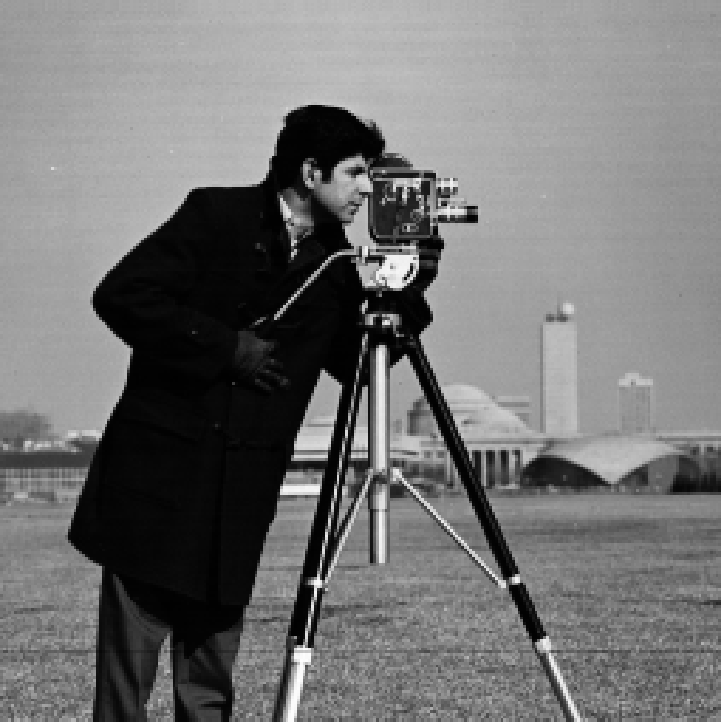
\includegraphics[width=0.45\textwidth]{figs/orig.png}};
        \node[above] at (image1.north) {Original};        
        % Image 2
        \node[anchor=south west,inner sep=0] (image2) at (0.55\textwidth,0) {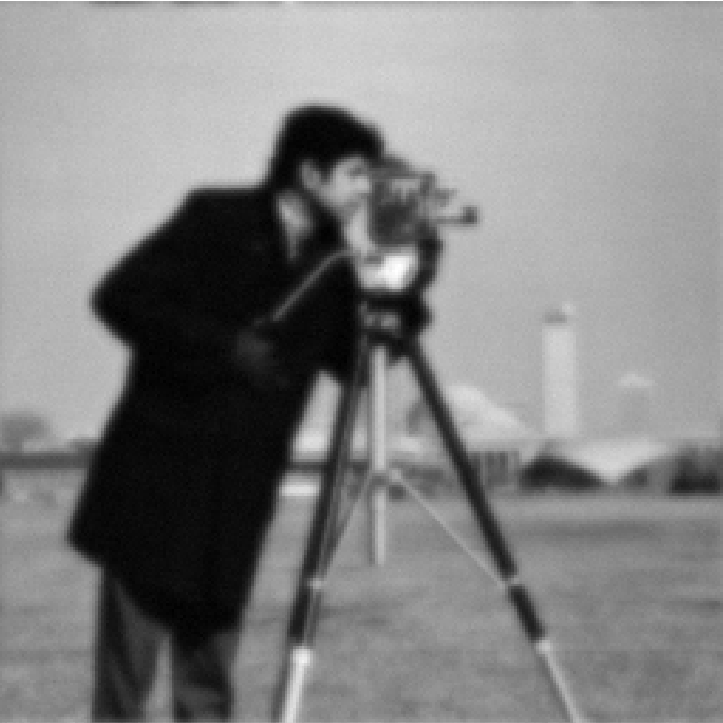
\includegraphics[width=0.45\textwidth]{figs/noisy.png}};
        \node[above] at (image2.north) {Blurred};
    \end{tikzpicture}
    \caption{Original and Blurred Cameraman Image.}
    \label{fig:combined}
\end{figure}


% Plot of f(u) vs iters
\begin{figure}
    \centering
    \begin{tikzpicture}
        % Image
        \node[anchor=south west,inner sep=0] (image) at (0,0) {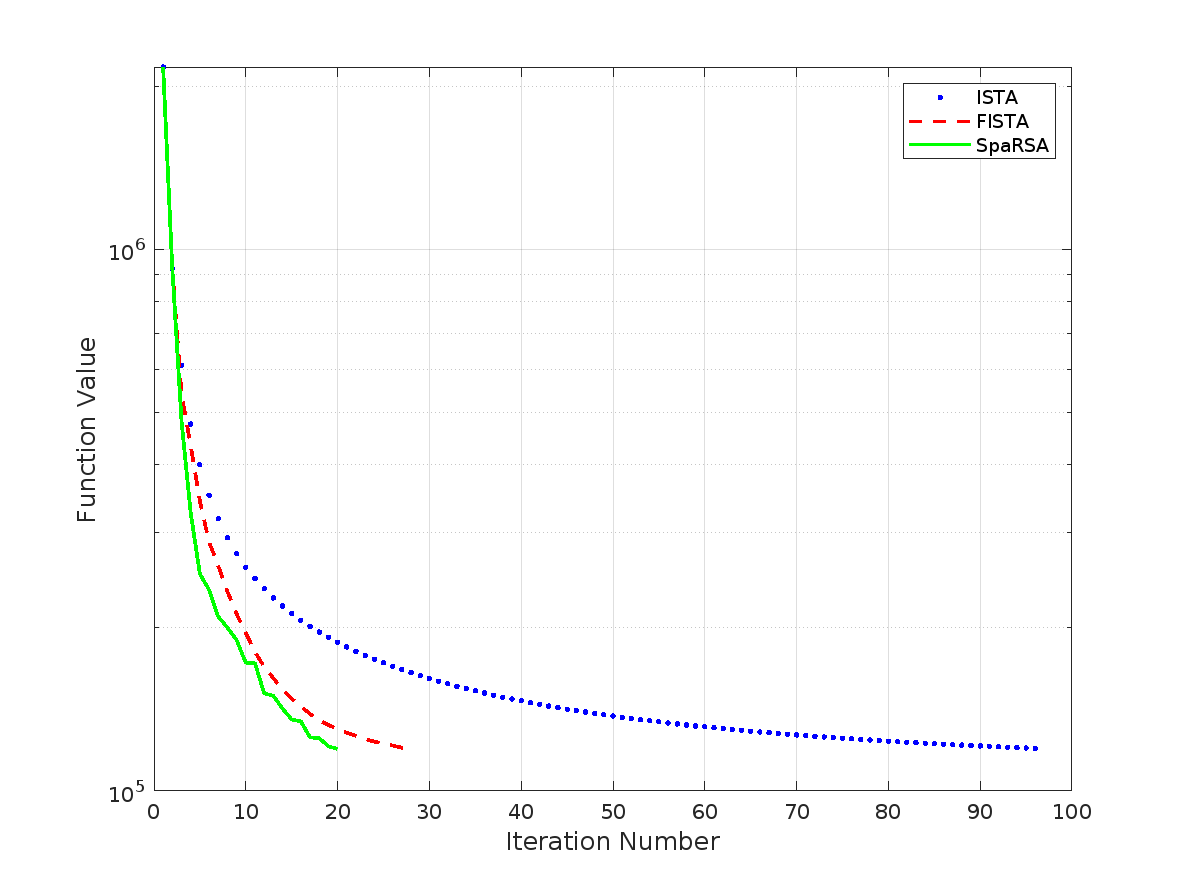
\includegraphics[width=0.8\textwidth]{figs/plot.png}};
    \end{tikzpicture}
    \caption{Function Value vs Iteration Number of ISTA, FISTA, and SpaRSA}
    \label{fig:combined}
\end{figure}

% Recovered from all 3 algs
\begin{figure}[H]
    \centering
    \begin{tikzpicture}
        % Image 1
        \node[anchor=south west,inner sep=0] (image1) at (0,0) {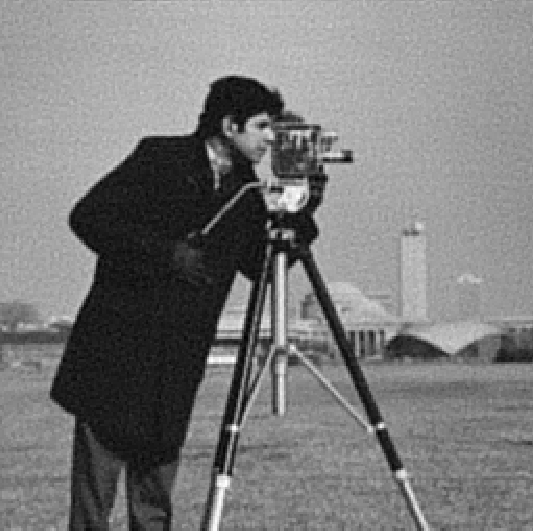
\includegraphics[width=0.3\textwidth]{figs/rec_ista.png}};
        \node[above] at (image1.north) {ISTA};        
        % Image 2
        \node[anchor=south west,inner sep=0] (image2) at (0.35\textwidth,0) {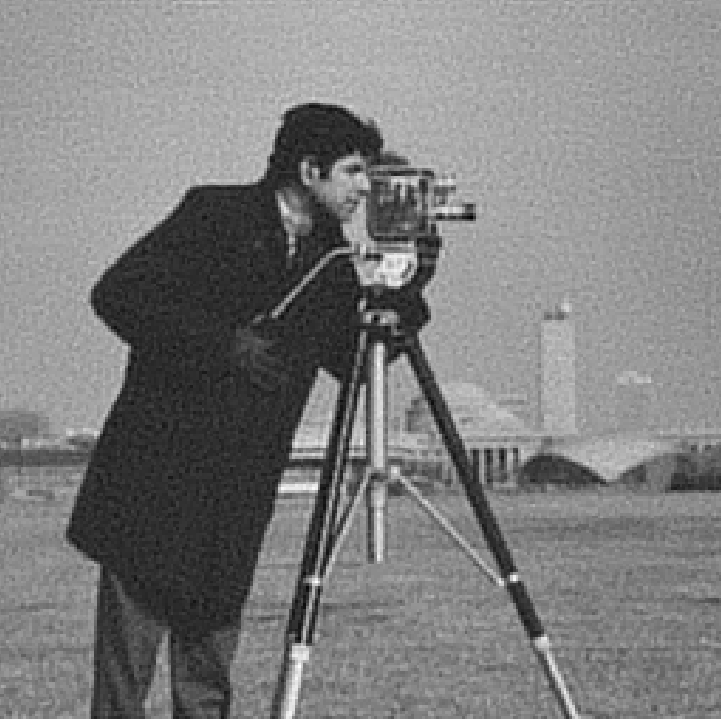
\includegraphics[width=0.3\textwidth]{figs/rec_fista.png}};
        \node[above] at (image2.north) {FISTA};        
        % Image 3
        \node[anchor=south west,inner sep=0] (image3) at (0.7\textwidth,0) {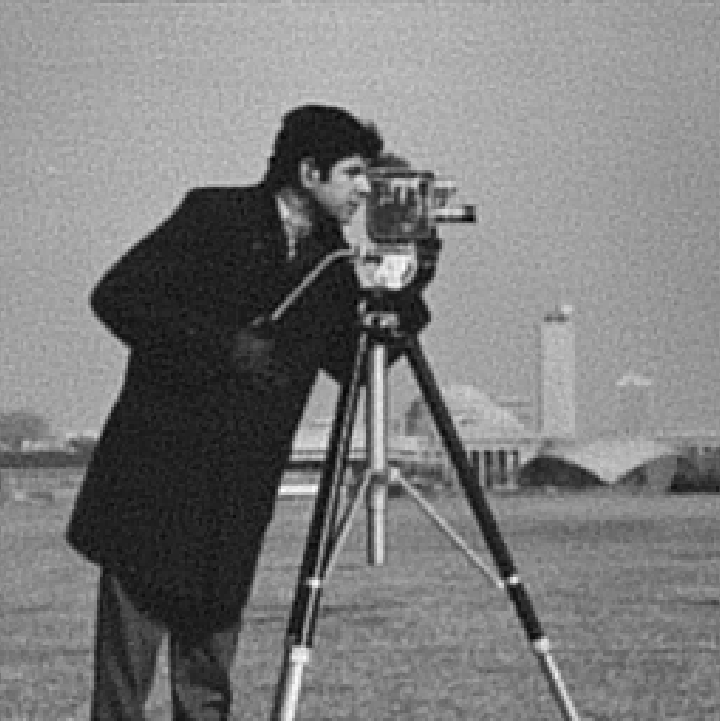
\includegraphics[width=0.3\textwidth]{figs/rec_sparsa.png}};
        \node[above] at (image3.north) {SpaRSA};
    \end{tikzpicture}
    \caption{Recovered Images from each Algorithm.}
    \label{fig:combined}
\end{figure}



% Plot grid comparing iterations
\begin{figure}[h]
    \centering
    \begin{tikzpicture}[every node/.style={inner sep=0pt,outer sep=0pt}]
        % Image 1
        \node (image1) at (0,0) {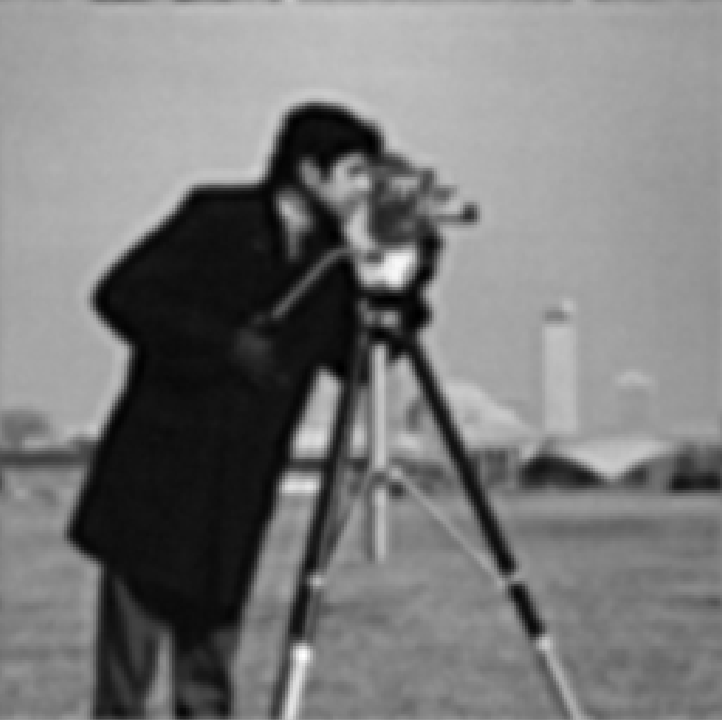
\includegraphics[width=0.3\textwidth]{figs/ISTA_5.png}};
        \node[above,yshift=5pt] at (image1.north) {ISTA: $F_5 = 3.99e5$};

        % Image 2
        \node (image2) at (0.35\textwidth,0) {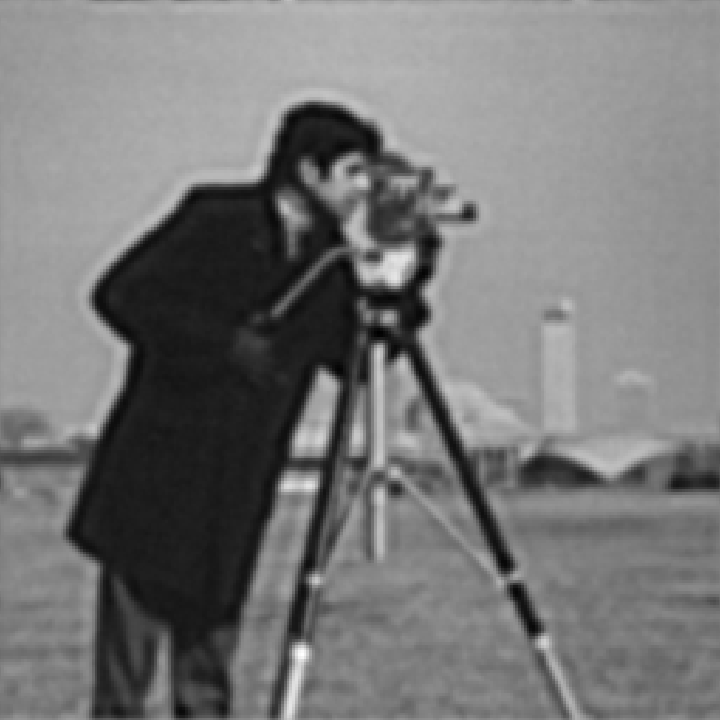
\includegraphics[width=0.3\textwidth]{figs/FISTA_5.png}};
        \node[above,yshift=5pt] at (image2.north) {FISTA: $F_5 = 3.42e5$};

        % Image 3
        \node (image3) at (0.7\textwidth,0) {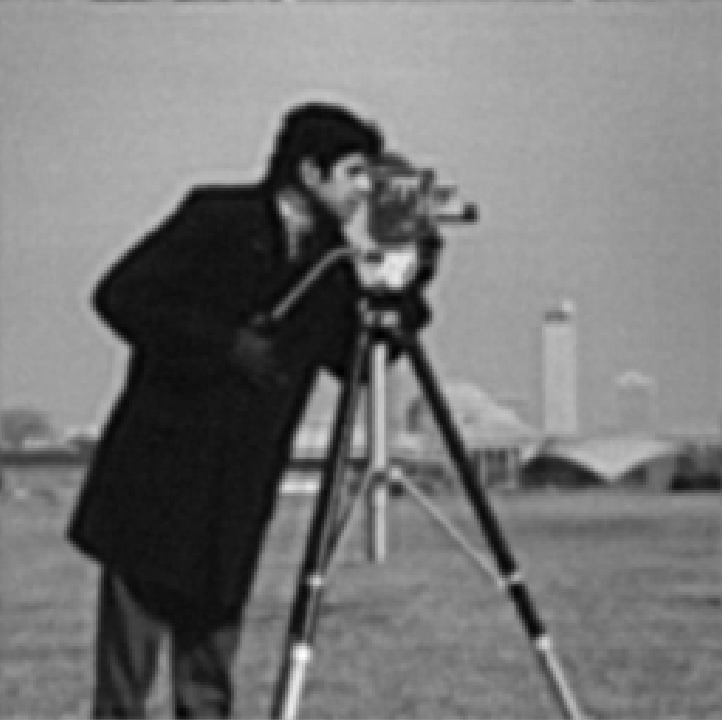
\includegraphics[width=0.3\textwidth]{figs/SPARSA_5.png}};
        \node[above,yshift=5pt] at (image3.north) {SpaRSA:$F_5 = 2.51e5$};

        % Image 4
        \node (image4) at (0,-0.35\textwidth) {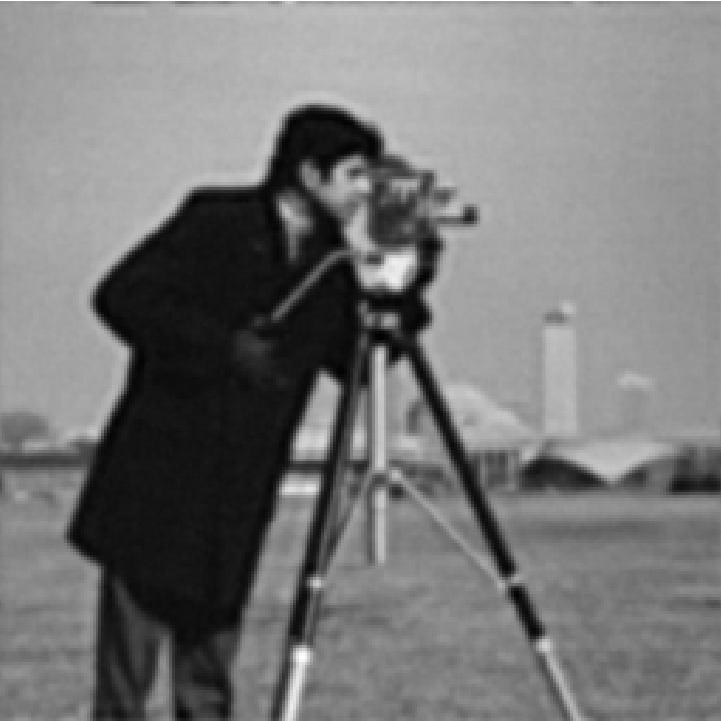
\includegraphics[width=0.3\textwidth]{figs/ISTA_10.png}};
        \node[above,yshift=5pt] at (image4.north) {ISTA: $F_{10} = 2.59e5$};

        % Image 5
        \node (image5) at (0.35\textwidth,-0.35\textwidth) {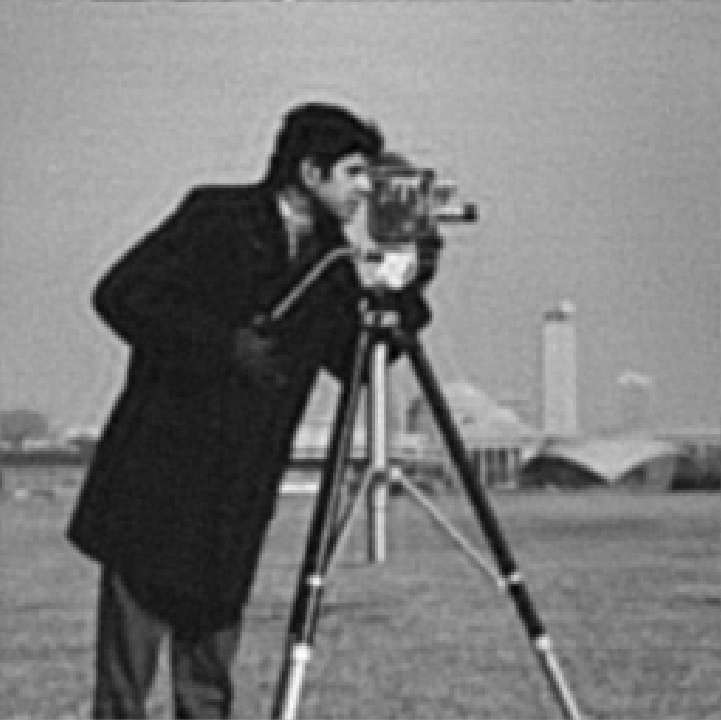
\includegraphics[width=0.3\textwidth]{figs/FISTA_10.png}};
        \node[above,yshift=5pt] at (image5.north) {FISTA: $F_{10} = 1.96e5$};

        % Image 6
        \node (image6) at (0.7\textwidth,-0.35\textwidth) {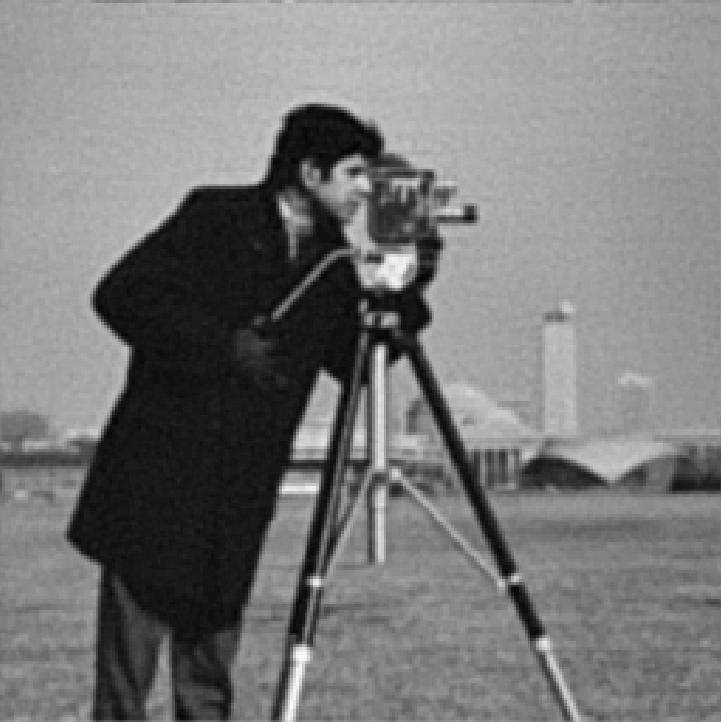
\includegraphics[width=0.3\textwidth]{figs/SPARSA_10.png}};
        \node[above,yshift=5pt] at (image6.north) {SpaRSA: $F_{10} = 1.72e5$};

        % Image 7
        \node (image7) at (0,-0.7\textwidth) {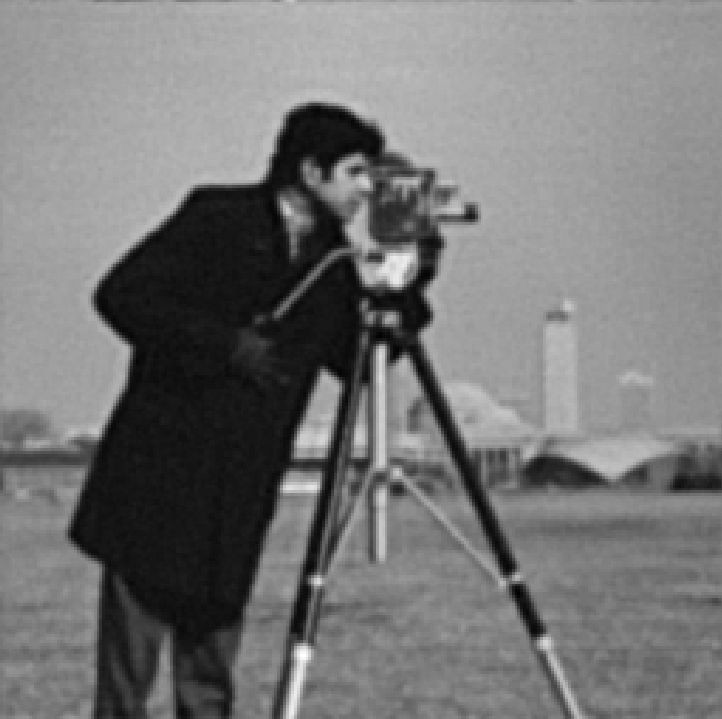
\includegraphics[width=0.3\textwidth]{figs/ISTA_20.png}};
        \node[above,yshift=5pt] at (image7.north) {ISTA: $F_{20} = 1.88e5$};

        % Image 8
        \node (image8) at (0.35\textwidth,-0.7\textwidth) {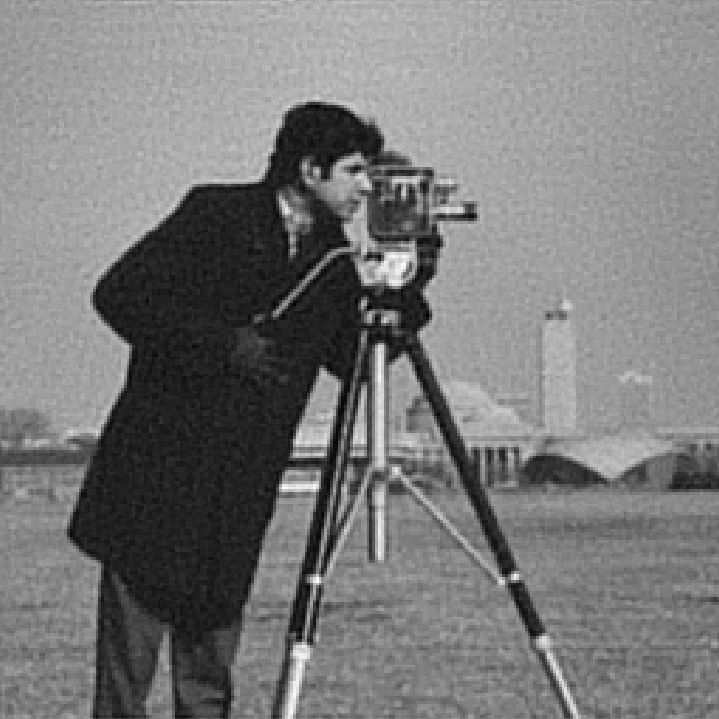
\includegraphics[width=0.3\textwidth]{figs/FISTA_20.png}};
        \node[above,yshift=5pt] at (image8.north) {FISTA: $F_{20} = 1.30e5$};

        % Image 9
        \node (image9) at (0.7\textwidth,-0.7\textwidth) {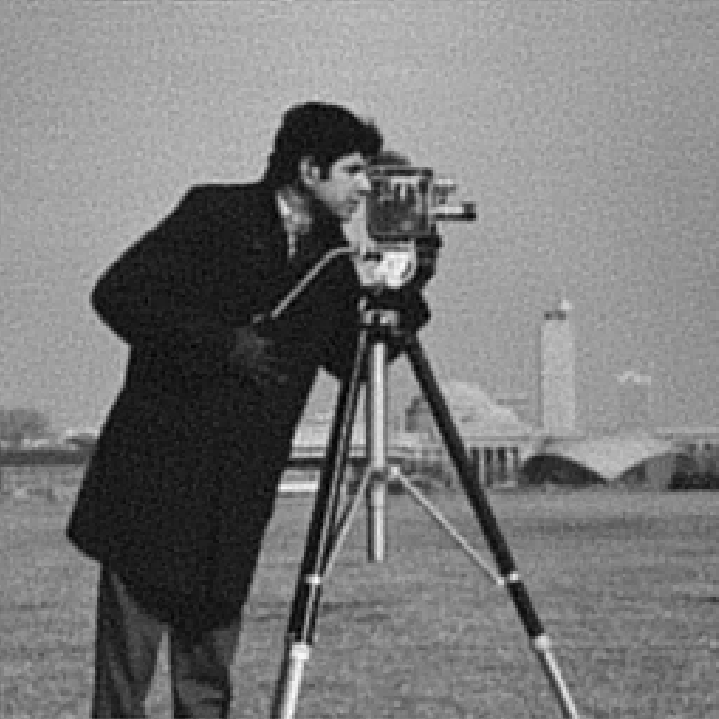
\includegraphics[width=0.3\textwidth]{figs/SPARSA_20.png}};
        \node[above,yshift=5pt] at (image9.north) {SpaRSA: $F_{20} = 1.19e5$};
    \end{tikzpicture}
    \caption{Outputs of ISTA, FISTA, and SpaRSA at selected iterations.}
    \label{fig:combined}
\end{figure}

\section{Conclusion}
We have discussed the proximal methods as a proxy of gradient based methods to the non-smooth objective function. We focused on the BPDN problem and two accelerated proximal methods proposed to enhance convergence speed of solving it. Our numerical experiments with explained FISTA \citep{beck2009fast} and SpaRSA \cite{wright2009sparse} algorithms verify the observations in the literature \citep{becker2011nesta, hager2011gradient} that the latter in practice converges faster than the former. The fundamental algorithms used for ISTA and SpaRSA were given by each respective publication, and the FISTA algorithm consisted of minor changes to ISTA. It should also be noted that the convergence analysis of SpaRSA is not presented, unlike that of FISTA.

\bibliography{refs}
\bibliographystyle{ieee}

\end{document}
